\chapter{Deep Multi-Agent RL Experiments}
Expanding on our the observations from the tabular experiments, we proceed to evaluate the better
performing algorithms under function approximation in large-scale 2p0s games to answer
question~\ref{qn3}.
For the neural experiments, we study the effect of NeuRD addition, and the utilization of
Optimistic-variants of popular optimizers (Optimistic-SGD, and Optimistic-Adam) when paired with
deep RL algorithms.
We do not evaluate extragradient updates for the Neural experiments.

\section{Experimental Domains}
For these experiments we choose three 2p0s EFGs, namely - Kuhn Poker, Abrupt Dark Hex, and Phantom
Tic-tac-toe.

\textbf{Kuhn Poker}
Kuhn Poker is a smaller extensive form game that allows for more introspection and exact
exploitability computation.

\textbf{Abrupt Dark Hex}
Abrupt Dark Hex

\textbf{Phantom Tic-Tac-Toe} Phantom Tic-Tac-Toe (Phantom TTT)

We train all the algorithms through self-play reinforcement learning.

\subsection{Approximate Exploitability}
For larger games, the computation of exact best responses to measure the exact exploitability is
prohibitive due to the large state space.
However, we can approximate the exploitability by training a local best response
agent~\cite{timbersApproximate2022} against the fixed joint policy that was trained through
self-play.
Then the exploitability can be approximated by sampling trajectories and measuring the average
reward the best response agent acheived against the exploited policy.
Let $\pi_{BR}$ be a learnt best-response approximator, and $\pi_{fixed}=(\pi_1, \pi_2)$ be the
exploitee-joint policy, then the approximate exploitability is given by:
\begin{equation}
	\label{eqn:appxexp} \text{Exp}_{appx} (\pi_{BR}, \pi_{fixed}) = \frac{1}{N} \left[ \sum_{i=1}^{N/2}
		\E_{a \sim \pi_1, \pi_{BR}} [R] + \sum_{i=1}^{N/2} \E_{a \sim \pi_{BR}, \pi_2} [R] \right]
\end{equation} \blue{TBD: rephrase the equation in terms of cumulative episodic rewards.
}

\subsection{Experiment Setup}
Our experiment setup is akin to that of~\cite{sokotaUnified2023}, we use
RLLib~\cite{liangRLlib2018} for implementing the algorithms, and interface with the game
implementations in OpenSpiel using RLLib's environment adapter.
For all the experiments we employ actor-critic version of the alogrithms without shared parameters
for the policy and value networks.
For all the experiments, we a use 2-layered MLP with (128, 128) hidden units.
We use GAE for computing the advantage estimates.
Please refer to the table~\ref{tab:hpes} in the appendix for a more exhaustive list of
hyperparameter values.
For Kuhn Poker, and Abrupt Dark Hex 2$\times$2, we train the agents in self-play for 1M steps and
measure exact exploitability at each iteration.
For Abrupt Dark Hex 3$\times$3, and Phantom TTT we train the agents for 5M steps and compute
approximate exploitability(~\ref{eqn:appxexp}) of the final joint-policy at the end of training.
We train a DQN agent against the fixed joint policy as the best-response appoximator $\pi_{BR}$,
for 5M steps, and evaluate its performance over $N$=1000 episodes.

\section{Results}

\ref{fig:neural1} plots the exact exploitabililty of the joint policy as a function of the
iterations.

\begin{figure}[H]
	\centering
	\begin{subfigure}[b]{0.6\textwidth}
		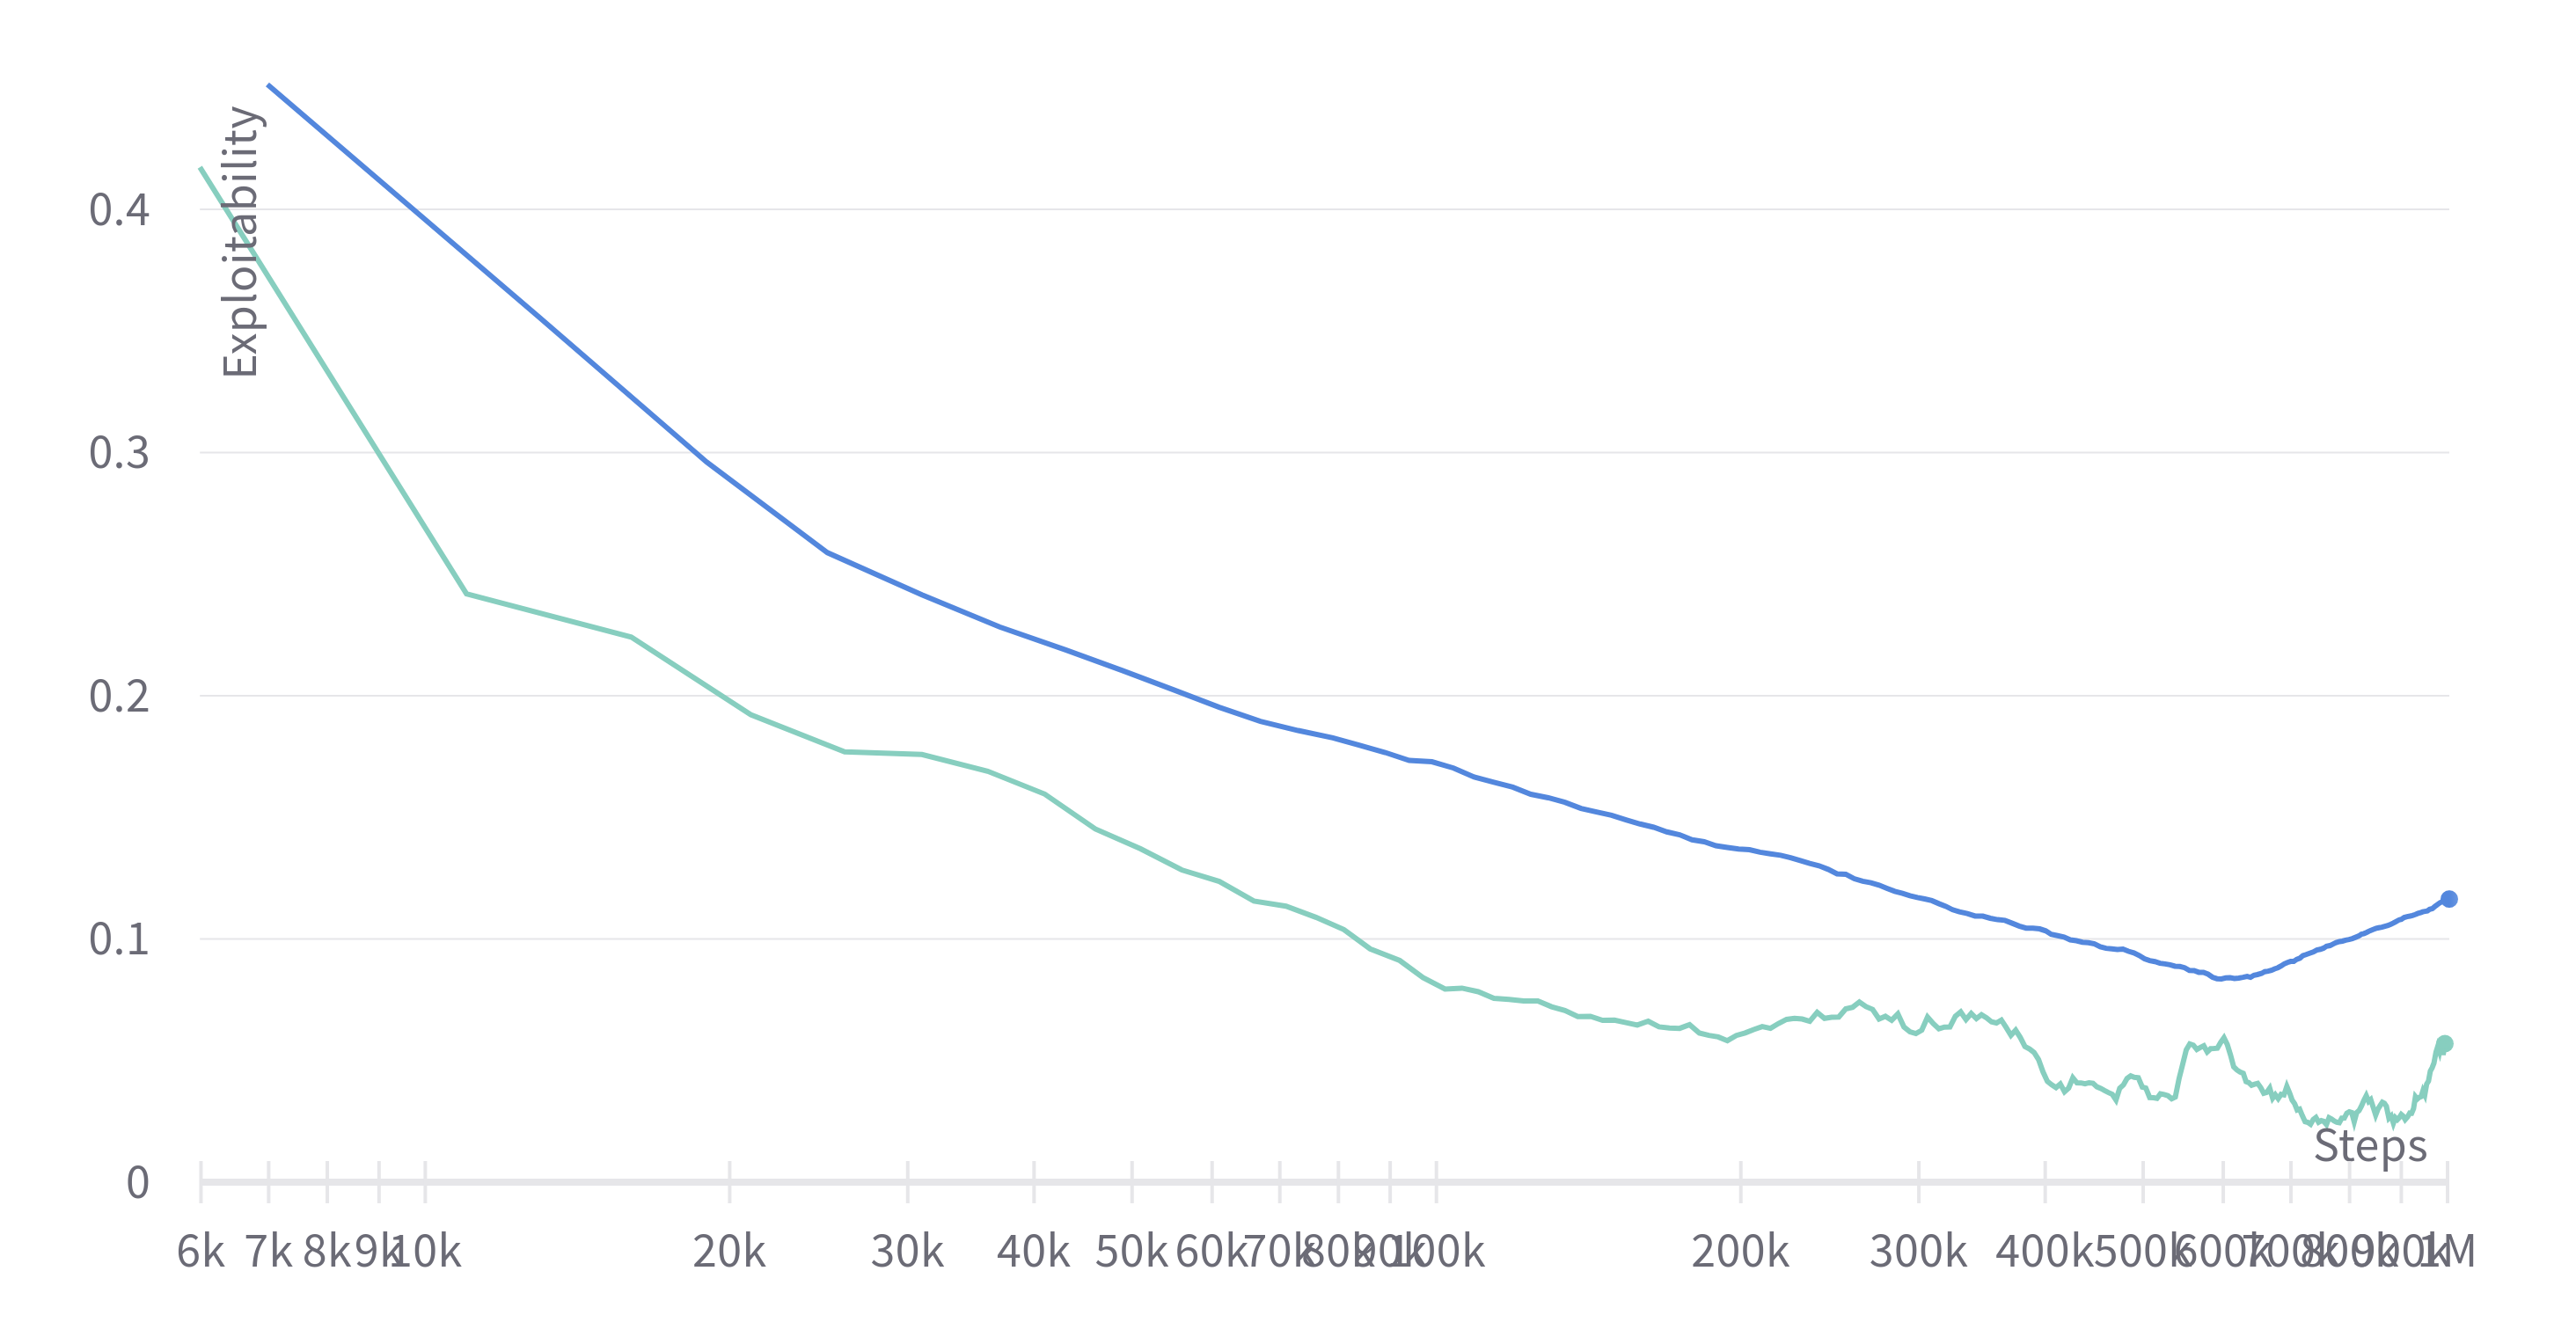
\includegraphics[width=\textwidth]{figs/kpoker.png}
		\caption{Kuhn Poker}
	\end{subfigure}
	\begin{subfigure}[b]{0.6\textwidth}
		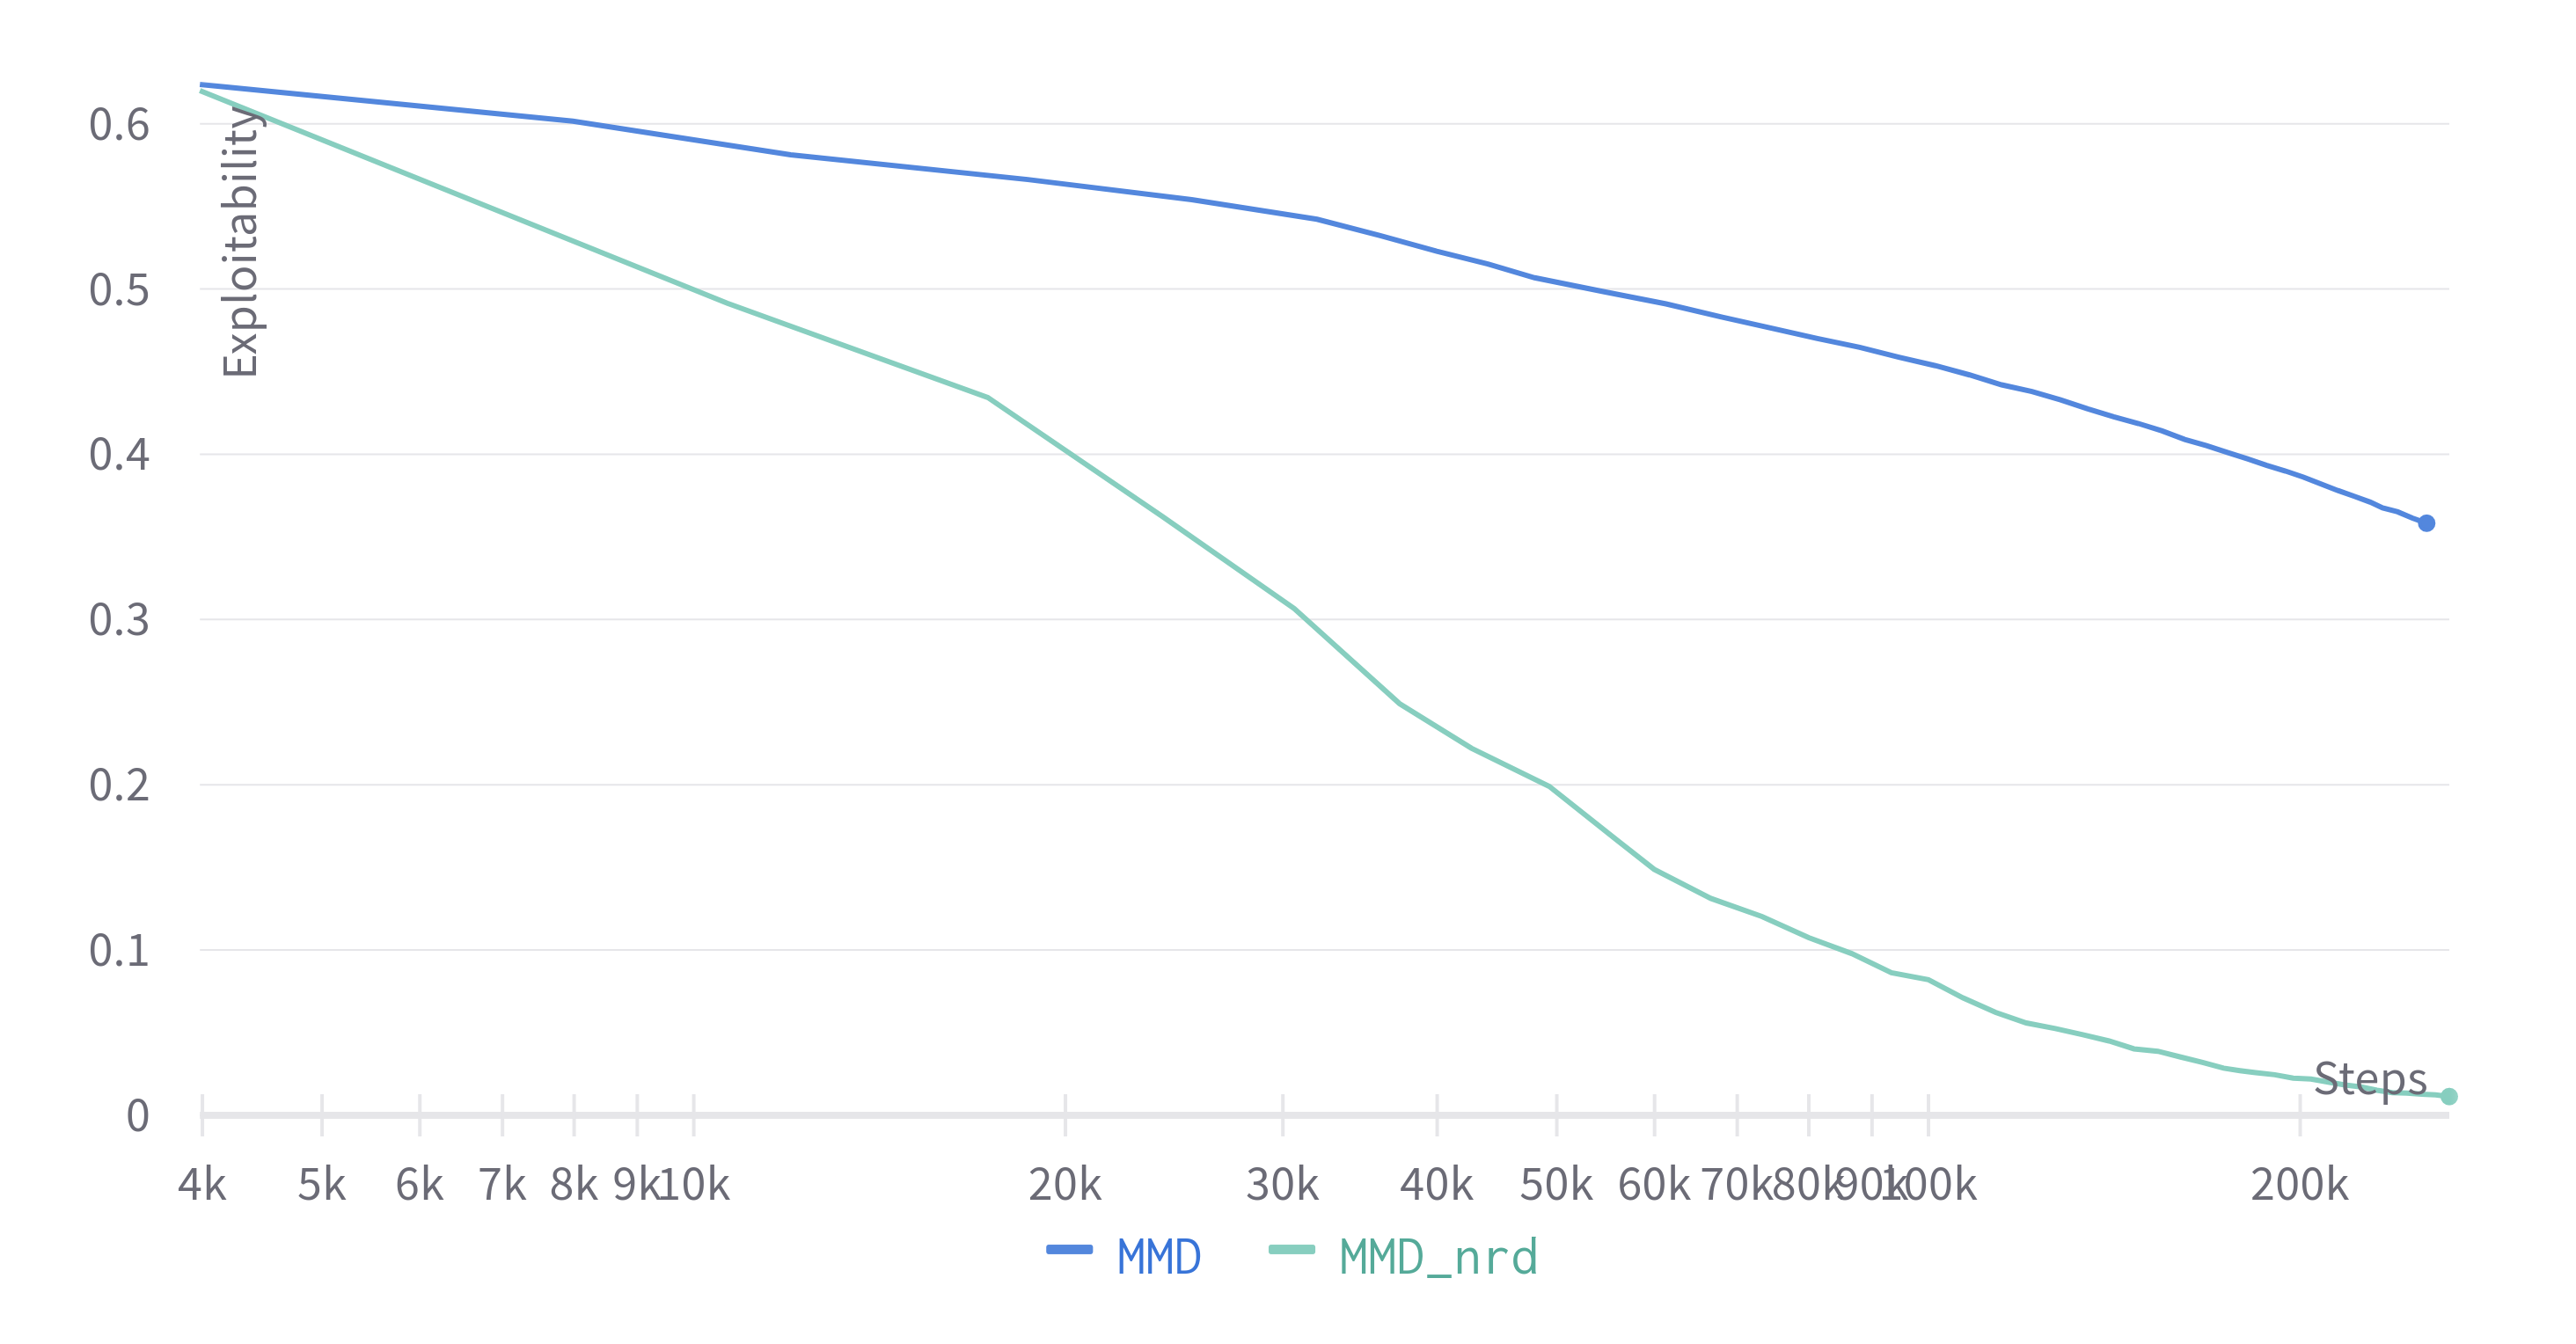
\includegraphics[width=\textwidth]{figs/ahex22.png}
		\caption{Abrupt Dark Hex (2$\times$2) (\red{1M steps version to be added})}
	\end{subfigure}
	\caption{Performance in small EFGs, measured by exact exploitability.}
	\label{fig:neural1}
\end{figure}

% We also compute approximate exploitability for the smaller games by training a DQN best-response
% agent for 1M steps against the fixed trained agents.

\ref{fig:neural2} shows improvement in performance by applying the NeuRD-fix in Abrupt Dark Hex
(3$\times$3) and Phantom TTT, as measured by the approximate exploitability.
\begin{figure}[H]
	\centering
	\begin{subfigure}[b]{0.4\textwidth}
		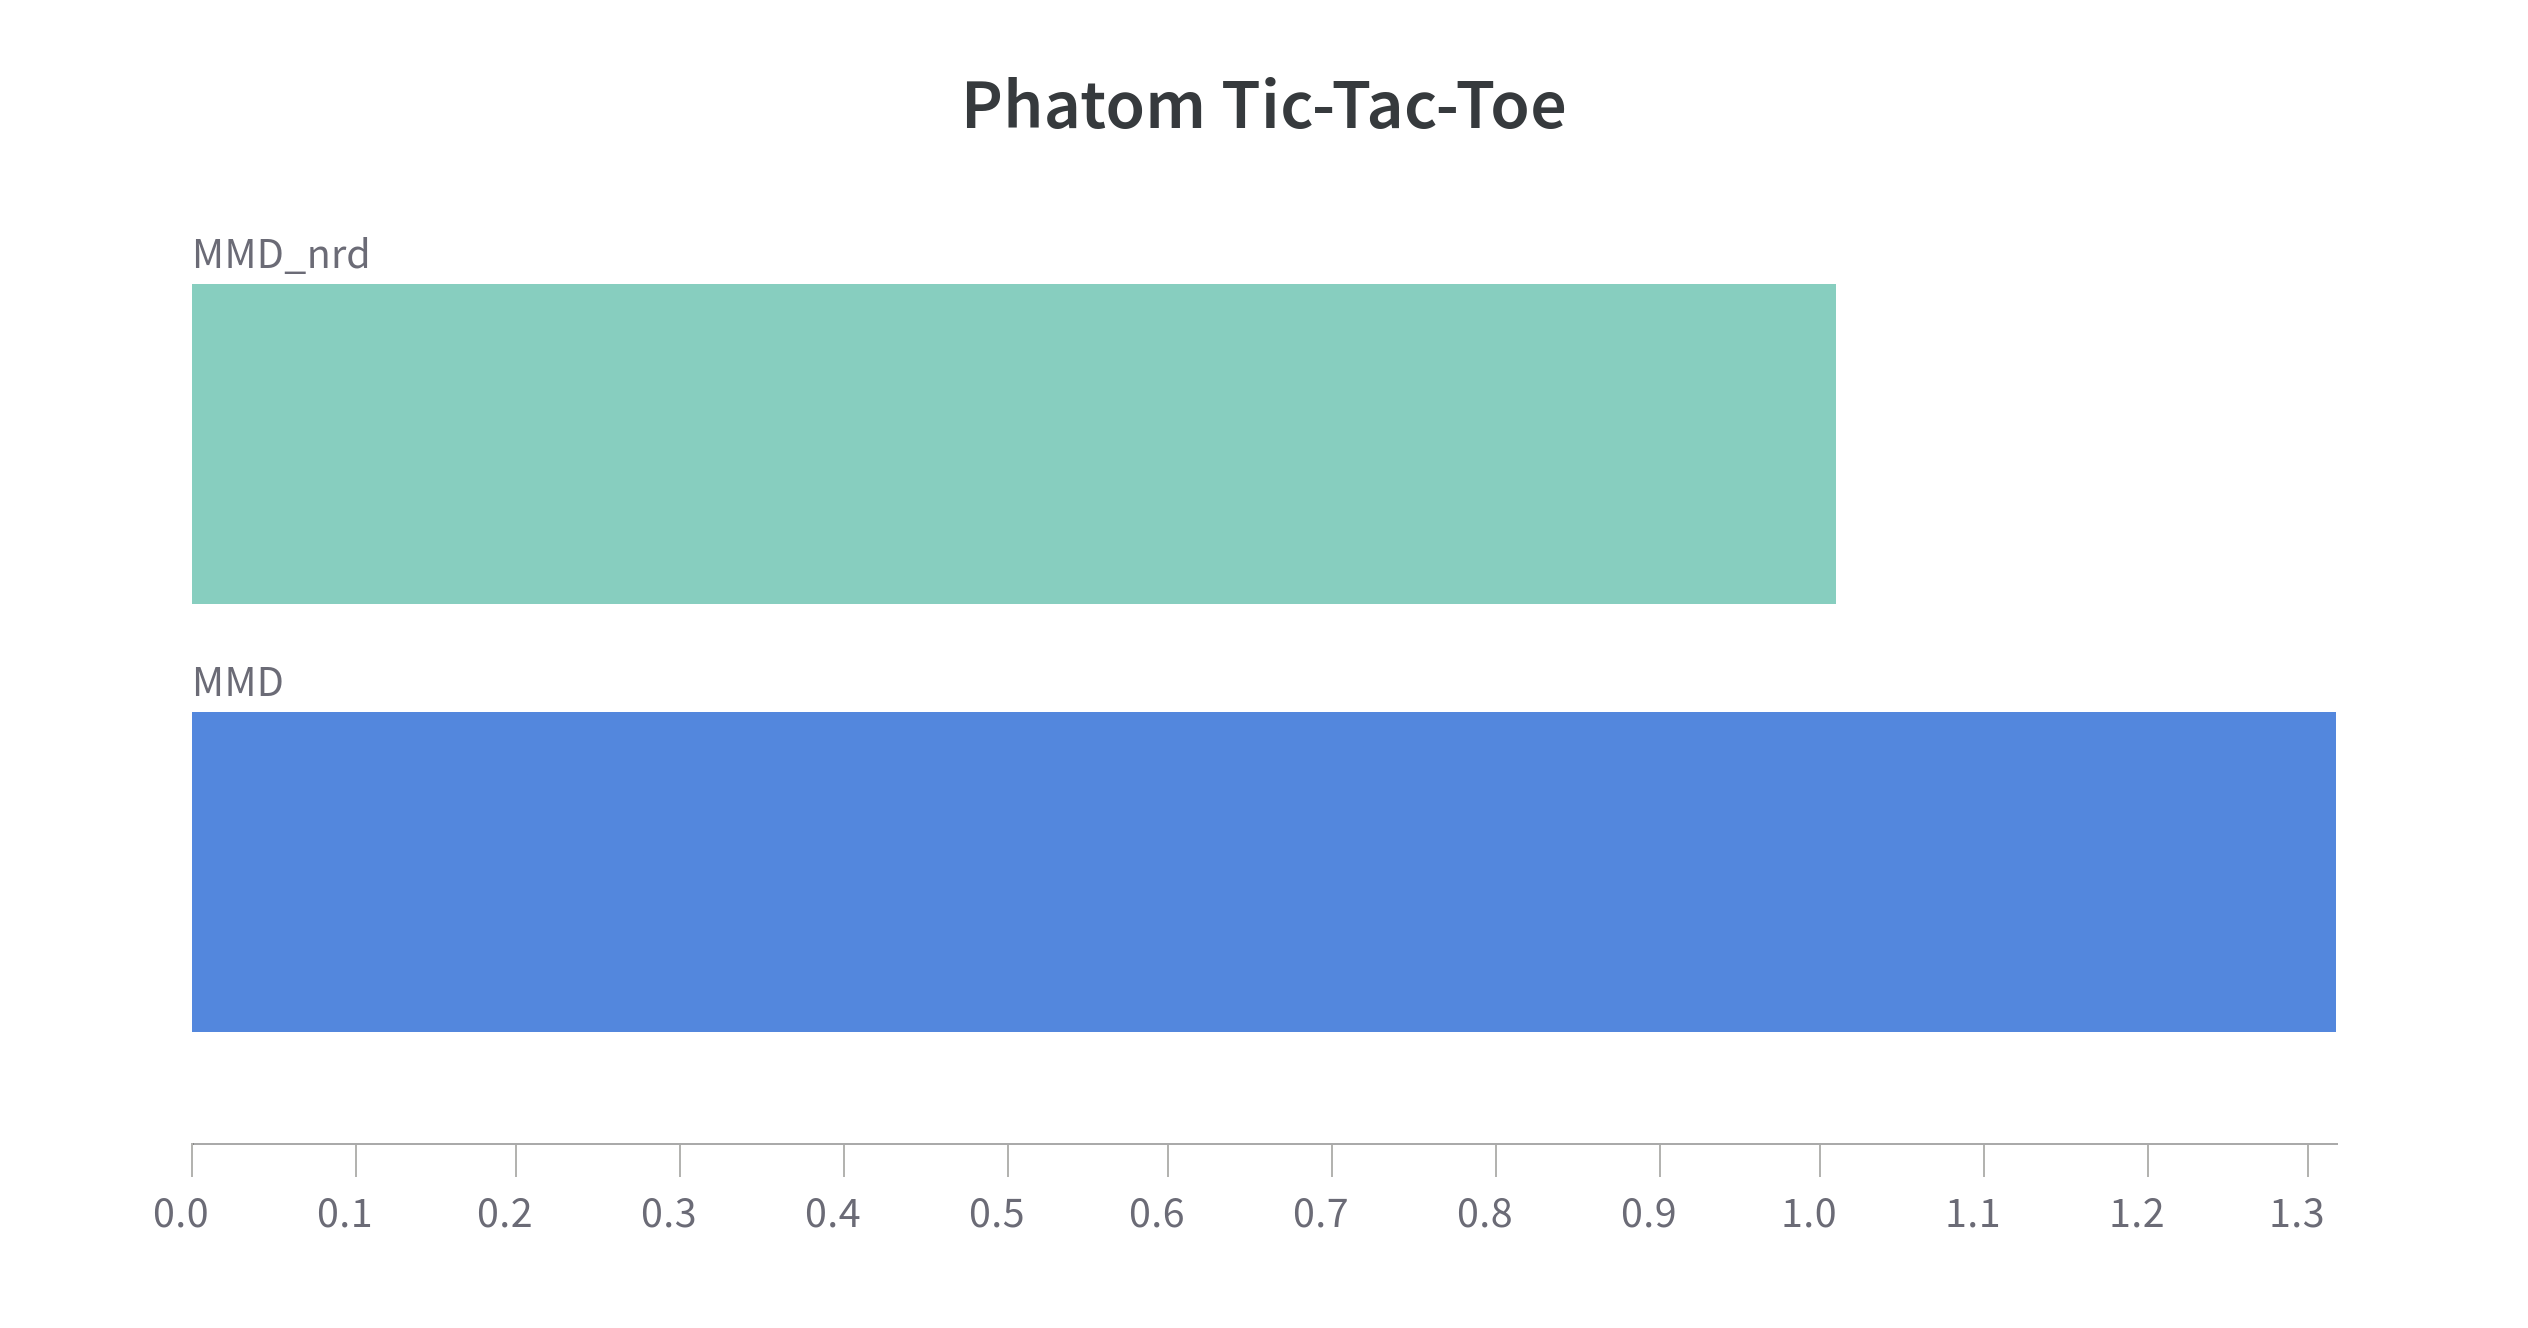
\includegraphics[width=\textwidth]{figs/pttt.png}
		\caption{Kuhn Poker}
	\end{subfigure}
	\begin{subfigure}[b]{0.4\textwidth}
		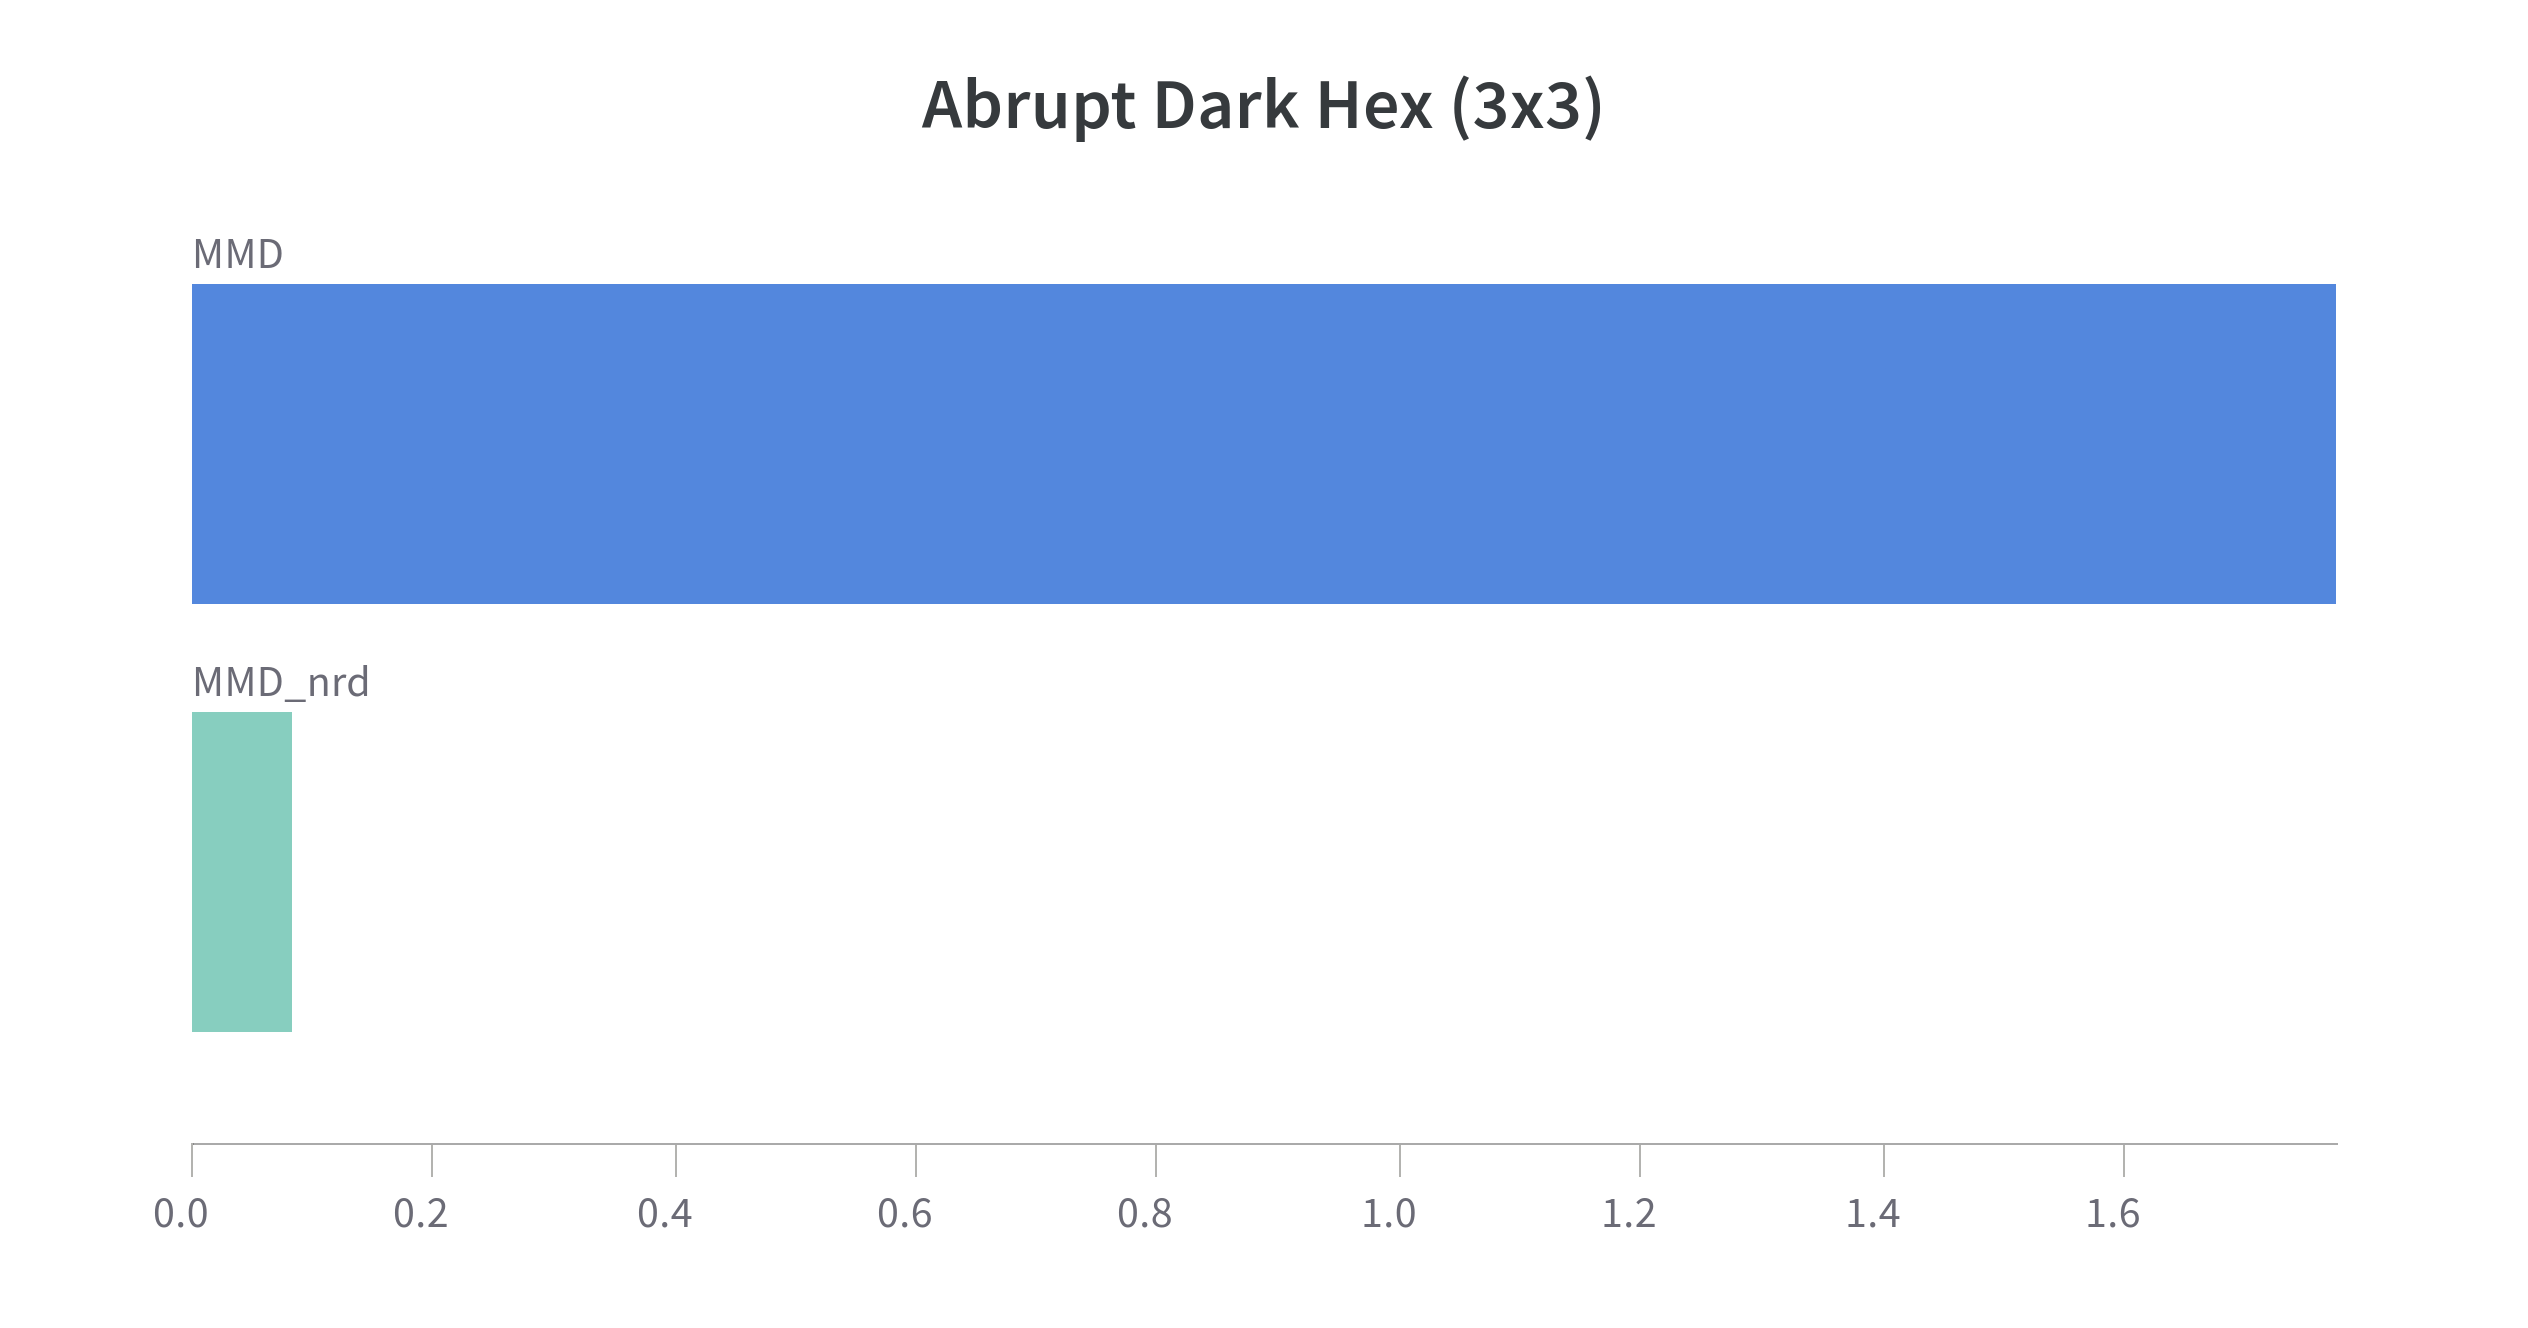
\includegraphics[width=\textwidth]{figs/ahex33.png}
		\caption{Abrupt Dark Hex (3$\times$3)}
	\end{subfigure}
	\caption{Performance in larger EFGs, measured by approximate exploitability.}
	\label{fig:neural2}
\end{figure}

\blue{We also evaluate these algorithms by having the trained agents play against each other in a
	head-to-head manner.}

\subsection{Observations}
\begin{itemize}
	\item {Similar to the tabular experiments, NeuRD-fix speeds up convergence of MMD in the Neural experiments as well.
	      }
\end{itemize}